\documentclass[../mathproblems.tex]{subfiles}
\graphicspath{{\subfix{../figures/}}}
\begin{document}
\chapter{AIME}
\section{2011-2020}
\subsubsection*{2016 AIME I/1} 
\textit{December 4, 2024}

For $-1<r<1$, let $S(r)$ denote the sum of the geometric series \[12+12r+12r^2+12r^3+\cdots .\]Let $a$ between $-1$ and $1$ satisfy $S(a)S(-a)=2016$. Find $S(a)+S(-a)$.

\textbf{Solution:}

We can see that $S(a) = 12+12a+12a^2+12a^3+\dots = \frac{12}{1-a}$.

We can also see that $S(-a)=12+12(-a)+12(-a)^2+12(-a)^3+\dots = \frac{12}{1+a}$.

So, $\frac{12}{1-a}\cdot \frac{12}{1+a}=\frac{144}{(1-a)(1+a)} = 2016$.

Now note that we are looking for $S(a)+S(-a) = \frac{12}{1-a}+\frac{12}{1+a}$. Simplifying this, we get $\frac{12(1+a)+12(1-a)}{(1-a)(1+a)} = \frac{24}{(1-a)(1+a)}$.

This looks similar to the equation above that equals $2016$, and we can see all we have to do is divide the equation by $6$, so $\frac{\frac{144}{(1-a)(1+a)}}{6} = \frac{2016}{6} = \boxed{336}$.

\noindent\hrulefill
\subsubsection*{2015 AIME II/14} 
\textit{November 18, 2024}

Let $x$ and $y$ be real numbers satisfying $x^4y^5+y^4x^5=810$ and $x^3y^6+y^3x^6=945$. Evaluate $2x^3+(xy)^3+2y^3$.

\textbf{Solution:}

We let $a=xy$ and $b=x+y$.

Factoring $x^4y^4+y^4x^5=810$ we get $(xy)^4(x+y)=810$ and substituting we get $(a^4)(b)=810$.

Factoring the other takes a little more steps.

When we factor $x^3y^6+y^3x^6$ we get $(xy)^3+(x^3+y^3)$.

Note that $(x+y)^3=x^3+y^3+3xy(x+y) \implies b^3=x^3+y^3+3ab$, so $x^3+y^3 = b^3-3ab$.

Therefore, factoring $x^3y^6+y^3x^6=945$ gets $(a^3)(b^3-3ab)=945$.

Note we are also looking for the value of $2(x^3+y^3)+(xy)^3$ or $2(b^3-3ab)+a^3$ or $2b(b^2-3a)+a^3$.

Dividing the two factored equations we get:
\begin{align*} \frac{(a^3)(b^3-3ab)}{(a^4)(b)}=\frac{945}{810} \\ \frac{a^3b^3-3a^4b}{a^4b} = \frac{945}{810}\\ \frac{b^2}{a}-3 = \frac{945}{810}\\ \frac{b^2}{a}-3 = \frac{7}{6}\\ \frac{b^2}{a}= \frac{25}{6} \end{align*}
Now for some manipulations.

Solving for $a$ we get $a=\frac{6}{25}b^2$.

I didn't know a better way to go from here, so I plugged it into the equation defined earlier, $(a^4)(b)=810$ to get
$\left(\frac{6}{25}b^2\right)^4(b)=810$.

After cheating with some desmos calculations this resulted in $\frac{1296}{390625}b^9=810$.

Solving for $b$ we get $b^9 = \frac{890\cdot 390625}{1296}$

Using some more online calculators for simplifying fractions, I got $b^9=\frac{1953125}{8}$. Now the cube root of $1953125$. Now $1953125$ looked like some power of $5$ so I assumed it was $5^9$ and desmos said it was correct! Happy Stasya!

So $b^3 = \sqrt[3]{\frac{1953125}{8}} = \frac{125}{2}$.

Now from earlier, there was the equation $a=\frac{6}{25}b^2$. We are looking for $a^3$ (we will look for $2b(b^2-3a)$ momentarily).

So we can take what we know and plug it into $a^3$:

\begin{align*} a^3 = \left(\frac{6}{25}b^2\right)^3 \\ = \frac{6^3}{25^3}b^6\\ = \frac{6^3}{25^3}b^3b^3\\ =\frac{6^3}{25^3}\frac{125}{2}\frac{125}{2} =\frac{6^3}{4} =54 \end{align*}We have found that $a^3 = 54$!

Ok now we need to find out $2b(b^2-3a)$ to finish the problem.

We can rewrite this as $2b^3-6ab$ to make this easier actually since we already know $b^3$.

We know that $a^3=54$, so we can plug that into one of the first equations we defined at the top, $(a^4)(b)=810$.

This results in $54ab=810$, so $ab=\frac{810}{54} = 15$.

Now we only need to plug these values in: $2\left(\frac{125}{2}\right) - 6(15) = 125-90 = 35$.

Adding $a^3 = 54$ with what I just found, we get $54+35 = \boxed{89}$.

\noindent\hrulefill

\subsubsection*{2015 AIME I/10}
\textit{December 8, 2024}

Let $f(x)$ be a third-degree polynomial with real coefficients satisfying \[|f(1)|=|f(2)|=|f(3)|=|f(5)|=|f(6)|=|f(7)|=12.\] Find $|f(0)|$. 

\textbf{Solution:}

We have this graph:
\begin{center}
    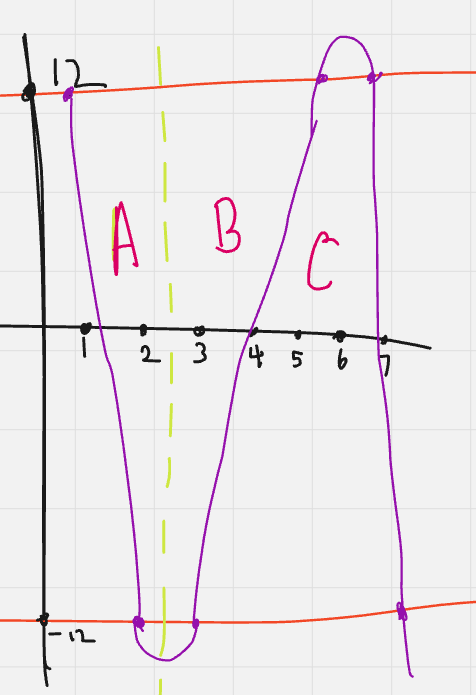
\includegraphics[width=0.4\textwidth]{GviFvqR.png}
\end{center}

From this, we see that for $3$ of these points $f(x)=12$ and the for the other three points we will have $f(x)=-12$.

In the regions $A$, $B$, and $C$, each region has a point where $f(x)=12$ and $f(x)=-12$, and we can see from the visual that $f(1)=f(5)=f(6)=12$ and $f(2)=f(3)=f(7)=-12$.

Now knowing that a cubic polynomial is in the form $f(x) = ax^3+bx^2+cx+d$, we can find what $f(0)$ is. Plugging in $0$, we find that $f(0)=d$. 

We can now set up a system of equations from the knowledge we know above.
\begin{align*}
a+b+c+d=12\\
8a+4b+2c+d=-12\\
27a+9b+3c+d=-12\\
125a+25b+5c+d=12\\
216a+36b+6c+d=12\\
343+49b+7c+d=-12
\end{align*}

Now since we have $4$ variables, we can just use the first four of these equations.

Subtracting the first equation from the second equation we get $7a+3b+c=-24$. Let's call this equation $5$.

Subtracting the first equation from the third equation we get $26a+8b+2c=-24$. Let's call this equation $6$.

Subtracting the first equation from the fourth equation we get $124a+24b+4c=0$. Let's call this equation $7$.

Now multiplying equation $5$ by $2$, we get $14a+6b+2c=-48$ and subtracting this from equation $6$, we get $6a+b=12$

Multiplying equation $6$ by $2$, we get $52a+16b+4c=-48$ and subtracting this from equation $7$, we get $9a+b=6$.

Now subtracting the two equations we just got, we can get $9a+b-(6a+b) = 3a = -6$, so $a=-2$.

Now plugging this back into $6a+b$, we get $-12+b=12$, so $b=24$.

Plugging $a$ and $b$ into equation $5$, we get $58+c=-24$. So $c=-82$.

Plugging this back into the first original equation, we get $-2+24-82+d=12$ so $d=12+60=\boxed{72}$.

\noindent\hrulefill

\subsubsection*{2012 AIME II/2}
\textit{December 12, 2024}

Two geometric sequences $a_1, a_2, a_3, \ldots$ and $b_1, b_2, b_3, \ldots$ have the same common ratio, with $a_1 = 27$, $b_1=99$, and $a_{15}=b_{11}$. Find $a_9$. 

\textbf{Solution:}

We have the two sequences $27,a_2,a_3,\dots$ and $99,b_2,b_3,\dots$. 

Since they have the same common ratio, we can just do $27r^{14} = 99r^{10}$, and we are looking for $27r^8$. 

When we divide the two, we get that $27r^4 = 99$, so $r^4 = \frac{99}{27} = \frac{11}{3}$. 

The answer is therefore $27\left(\frac{11}{3}\right)\left(\frac{11}{3}\right) = 3\cdot 121 = \boxed{363}$.

\noindent\hrulefill

\subsubsection*{2012 AIME I/2}
\textit{December 6, 2024}

The terms of an arithmetic sequence add to $715$. The first term of the sequence is increased by $1$, the second term is increased by $3$, the third term is increased by $5$, and in general, the $k$th term is increased by the $k$th odd positive integer. The terms of the new sequence add to $836$. Find the sum of the first, last, and middle terms of the original sequence. 

\textbf{Solution:}

Let the arithmetic sequence be $a_1 + a_2 + a_3 + \dots + a_n = 715$.

We also have $(a_1+1) + (a_2 + 3) + (a_3 + 5) + (a_n+(2n-1)) = 836$.

Notice that the first arithmetic sequence is in the second arithmetic sequence. We can rewrite the second arithmetic sequence as 
\[ (a_1 + a_2 + a_3 + \dots + a_n) + (1 + 3 + 5 + \dots + (2n-1))\]
Which is also $715 + (1+3+5+\dots+(2n-1))=836$.

Note that the sum $(1+3+5+\dots+(2n-1))=n^2$. Therefore we have $n^2 = 836-715 = 121$. We now have $n=11$.

Now we are looking for the sum of $a_1+a_6+a_{11}$. We know that $a_6$ will be the average of $a_1$ and $a_{11}$, so from that we know that $a_1+a_{11} = 2a_6$.

Now if we continue the average of $a_2$ and $a_{10}$ will also be $a_6$ so the sum of $a_2$ and $a_{10}$ is $2a_6$.

If we continue this, we should see that the sum of $a_1 + a_2 + a_3 + \dots + a_{11} = 735$ will just be equivalent to $11a_6 = 735$. 

Note that $a_1+a_{11}+a_6 = 2a_6 + a_6 = 3a_6$, so we can just multiply $735$ by $11a_6=735$ by $\frac{3}{11}$ to get $3a_6=715\left(\frac{3}{11}\right) = \boxed{195}$.

\noindent\hrulefill

\subsubsection*{2010 AIME I/9} 
\textit{November 25, 2024}

Let $(a,b,c)$ be a real solution of the system of equations $x^3 - xyz = 2$, $y^3 - xyz = 6$, $z^3 - xyz = 20$. The greatest possible value of $a^3 + b^3 + c^3$ can be written in the form $\frac {m}{n}$, where $m$ and $n$ are relatively prime positive integers. Find $m + n$.

\textbf{Solution:}

Ok pretty much let $a=x$, $b=y$, and $c=z$.

Then we have
\[ a^3=2+abc \qquad b^3=6+abc \qquad c^3=20+abc \]
Also adding these we have $a^3+b^3+c^3=28+3(abc)$.

So we can like substitute $r=abc$ and then multiply the first rewritten equations above so:
\begin{align*} a^3 = 2+r\\ b^3 = 6+r\\ c^3 = 20+r \end{align*}Multiplying these, we get
$(abc)^3=r^3=(2+r)(6+r)(20+r)$.

Ok now we can just expand:
\begin{align*} r^3=(12+2r+6r+r^2)(20+r)\\ r^3=240+12r+160r+8r^2+20r^2+r^3\\ 0=240+12r+160r+8r^2+20r^2\\ 0=28r^2+172r+240\\ 0=7r^2+43r+60 \end{align*}The factors that multiply to $420$ that add up to $43$ are $28$ and $15$, so this can be factored to $(7r+15)(r+4)$.

Therefore, $r=-\frac{15}{7}$ and $r=-4$.

Above, we see that $a^3+b^3+c^3=28+3r$, so since both values of $r$ are negative, the negative number closer to 0 will maximize the value.

Therefore, $r=-\frac{15}{7}$.

Plugging this in, we get $a^3+b^3+c^3 = 28+3\left(-\frac{15}{7}\right)$.

Expanding this, we get $\frac{151}{7}$, so $151+7=\boxed{158}$.

\noindent\hrulefill
\section{2000-2010}
\subsubsection*{2007 AIME I/2} 
\textit{November 29, 2024}

A 100 foot long moving walkway moves at a constant rate of 6 feet per second. Al steps onto the start of the walkway and stands. Bob steps onto the start of the walkway two seconds later and strolls forward along the walkway at a constant rate of 4 feet per second. Two seconds after that, Cy reaches the start of the walkway and walks briskly forward beside the walkway at a constant rate of 8 feet per second. At a certain time, one of these three persons is exactly halfway between the other two. At that time, find the distance in feet between the start of the walkway and the middle person.

\textbf{Solution:}

Ah well Al ends up going 6 ft/sec, Cy goes 8 ft/sec and Bob ends up going 10 ft/sec.

So like pretty early on, we can find that Al will end up somewhere in between Cy and Bob, eventually Al will fall behind, but at earlier times it can be assumed that Al will end up halfway between Cy and Bob.

Therefore we have $\frac{8(t-4)+10(t-2)}{2} = 6t$.

Solving for $t$ we get $8t-32+10t-20=12t$ and $6t=52$, so $t=\frac{52}{6}=\frac{26}{3}$.

Substituting this into $6t$ for Al, we get $6\left(\frac{26}{3}\right) = \boxed{52}$.

\noindent\hrulefill
\subsubsection*{2006 AIME II/1} 
\textit{October 25, 2024}

In convex hexagon $ABCDEF$, all six sides are congruent, $\angle A$ and $\angle D$ are right angles, and $\angle B, \angle C, \angle E,$ and $\angle F$ are congruent. The area of the hexagonal region is $2116(\sqrt{2}+1).$ Find $AB$.

\textbf{Solution:}

When we draw the diagram, we get a 45-45-90 triangle with a rectangle and a 45-45-90 triangle again on the top of the rectangle.

From this, we can find the area of the rectangle - so the area of the rectangle is $x(x\sqrt{2})$. The two 45-45-90 triangles create a square, so the area is $x^2$ so the area of convex hexagon is $x(x\sqrt{2})+x^2$. 

Simplifying, we get $x^2(\sqrt{2}+1)$. From the given statement in the question, we can find that $x^2=2116$, so $x=\boxed{46}$. 

\noindent\hrulefill

\subsubsection*{2005 AIME II/3}
\textit{December 12, 2024}

An infinite geometric series has sum 2005. A new series, obtained by squaring each term of the original series, has 10 times the sum of the original series. The common ratio of the original series is $\frac mn$ where $m$ and $n$ are relatively prime integers. Find $m+n.$ 

\textbf{Solution:}

We let the first sequence be $a,ar,ar^2,\dots$ and the second sequence be $(a)^2, (ar)^2, (ar^2)^2,\dots$. The second sequence can be written as $a^2, a^2r^2, a^2r^4,\dots$ now.

From this we can see that for the first sequence the sum is $\frac{a}{1-r}=2005$, and for the second sequence it is $\frac{a^2}{1-r^2}=2005\cdot 10 = 20050$.

Now it is much easier to think about both of these in terms of just $r$, since that is what we are trying to find.

We can actually simplify $\frac{a^2}{1-r^2}$ by substituting the sum of the first sequence. So we have ${a\cdot a}{(1+r)(1-r)}$. From this we can see we can substitute $2005$ in, so $\frac{2005a}{1+r} = 20050$. And now dividing, we get that $\frac{a}{1+r} = \frac{20050}{2005} = 10$.

Now with these two equations we can set them equal to each other. First we have $a = 2005(1-r) = 2005-2005r$ from the first sequence and $a = 10(1+r) = 10+10r$ from the second sequence. 

Setting these equal to each other we get that $2005-2005r=10+10r$ or $2015r = 1995$. Therefore $r=\frac{1995}{2015} = \frac{399}{403}$. The answer is therefore $399+403 = \boxed{802}$. 

\noindent\hrulefill



\subsubsection*{2001 AIME I/3} 
\textit{November 23, 2024}

Find the sum of the roots, real and non-real, of the equation $x^{2001}+\left(\frac 12-x\right)^{2001}=0$, given that there are no multiple roots.

\textbf{Solution:}

Let $a=x-\frac{1}{4}$.

Then we have
\[ \left(\frac{1}{4}+a\right)^{2001} + \left(\frac{1}{4}-a\right)^{2001} = 0\]
The binomial theorem states that $(a+b)^n = \sum_{k=0}^n \binom{n}{k} a^{n-k}b^k$

Expanding both terms we get

\[ \left(\frac{1}{4}+a\right)^{2001} = \sum_{k=0}^{2001} \binom{2001}{k}\left(\frac{1}{4}\right)^{2001-k}a^k\]and
\[ \left(\frac{1}{4}-a\right)^{2001} = \sum_{k=0}^{2001} \binom{2001}{k}\left(\frac{1}{4}\right)^{2001-k}(-a)^k\]
Adding these two together, we get
\[ \sum_{k=0}^{2001} \binom{2001}{k}\left(\frac{1}{4}\right)^{2001-k} (a^k+(-a)^k)\]
Note that $a^k+(-a)^k$ will be equal to zero when $k$ is an odd number, so only when $k$ is an even number will there be a non-zero value and that it will result in $2a^k$ given an even $k$.

We therefore get:
\[ 2\sum_{k=0}^{2001} \binom{2001}{k}\left(\frac{1}{4}\right)^{2001-k} a^k = 0\]
Therefore the second term will have an odd power, and therefore a coefficient of $0$. Therefore by Vieta's, the sum of the roots will be $0$ divided by something, or $0$.

Because the highest power will be $2000$, then there are $2000$ roots. Substituting back to the original equation, we can see that $a = x-\frac{1}{4}$. The sum of the roots of $x$ will be the sum of the roots of $a+2000\cdot\frac{1}{4}$ or $\boxed{500}$.

\noindent\hrulefill
\section{Before 2000}
\subsubsection*{1998 AIME/3}
\textit{December 9, 2024}

The graph of $y^2 + 2xy + 40|x|= 400$ partitions the plane into several regions. What is the area of the bounded region? 

\textbf{Solution:}
Isolating the $40|x|$ term, we get that $400-y^2-2xy = 40|x|$.

Then we have two cases:

Case 1:
$40x = 400-y^2-2xy$

Case 2:
$40x = -400+y^2+2xy$

In the first case - 
\begin{align*}
40x = 400-y^2-2xy\\
40x+2xy = 400-y^2\\
2x(20+y) = (20-y)(20+y)
\end{align*}
We can see that when $y=-20$, then the two equations are equal. When we cancel out the $(20+y)$ term, we can see that $2x=20-y$, or $y=-2x+20$.

For the second case - 
\begin{align*}
40x = -400+y^2+2xy\\
40x-2xy = -400+y^2\\
-2x(y-20) = (y-20)(y+20)
\end{align*}
Here, we can see that $y=20$ will result in both equations being the same. When cancelling out the $(y-20)$ term, then we have $-2x=y+20$, so $y=-2x-20$.

When we graph the 4 lines, we have the following graph
\begin{center}
    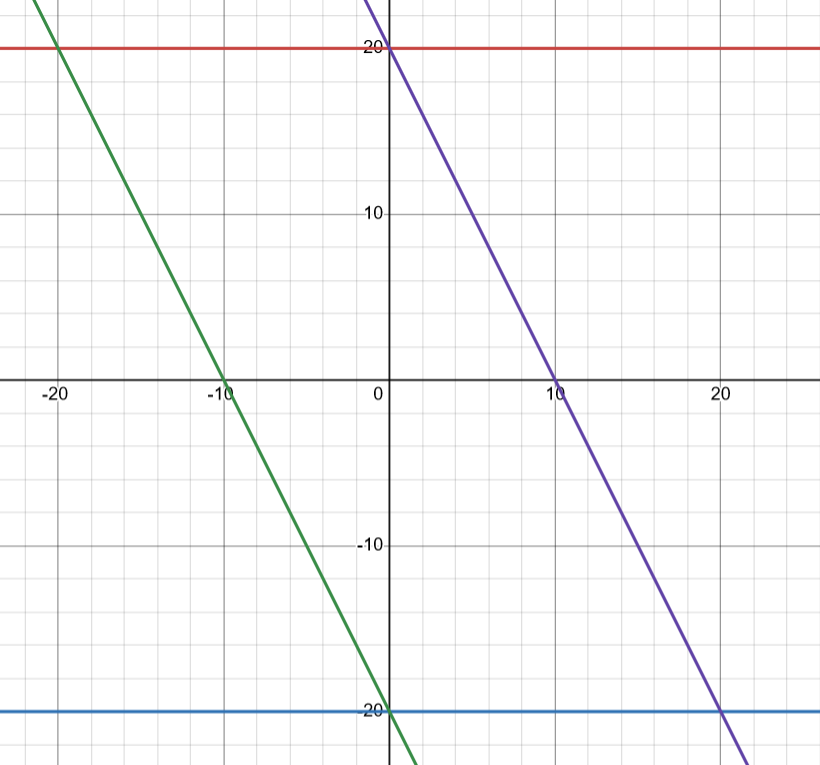
\includegraphics[width=0.4\textwidth]{tjd4v81.png}
\end{center}

The height of this shape is $40$ and the base is $20$, so $40\cdot 20 = \boxed{800}$.

\noindent\hrulefill


\subsubsection*{1991 AIME/1} 
\textit{November 21, 2024}

Find $x^2+y^2_{}$ if $x_{}^{}$ and $y_{}^{}$ are positive integers such that \begin{align*} xy+x+y&=71, \\ x^2y+xy^2&=880. \end{align*}

\textbf{Solution:}

Let $a=xy$ and $b=x+y$.

By substituting these variables in, we get $a+b=71$ and $ab = 880$.

We can solve for $a$ by rearranging $a+b = 71$ to $b=71-a$.

Substituting this into the second equation, we get $a(71-a)=880$.

This simplifies to $a^2-71a-880$.

Factoring this, we get $(a-16)(a-55)$, so $a=16,55$.

We can show that $a\neq 16$ because in this case, it would mean that $x+y=55$, and there are no two factors that add up to 55 and can multiply to 16.

So, $a=55$ or $xy=55$, so $(x,y)$ is $(11,5)$ or $(5,11)$.

Therefore, $5^2+11^2=\boxed{146}$.

\noindent\hrulefill
\end{document}